\documentclass[12pt]{report}
\setlength{\topmargin}{-1in}
\setlength{\textheight}{9.8in}
\setlength{\oddsidemargin}{.125in}
\setlength{\textwidth}{6.8in} 
\setlength{\parindent}{3em}
\pretolerance=150
\newcommand{\cm}[1]{\par\textbf{{#1}}\par}
\newcommand{\nosection}[1]{\addcontentsline{toc}{section}{{#1}}\section*{{#1}}}
%\usepackage[ natbib=true, style=numeric, sorting=none ]{biblatex}
%\addbibresource{../library.bib}
\usepackage[table,svgnames]{xcolor}
\usepackage{multicol}
\usepackage{fancyvrb}
\usepackage{tikz}
\usepackage{pgfplots} 
\usepackage{pgfgantt}
\usepackage{pdflscape}
\pgfplotsset{compat=newest} 
\pgfplotsset{plot coordinates/math parser=false}
\RecustomVerbatimCommand{\VerbatimInput}{VerbatimInput}{
  fontsize=\footnotesize % default
  %
  frame=lines,  % top and bottom rule only
  framesep=2em, % separation between frame and text
  rulecolor=\color{Gray},
  %
  label=\fbox{\color{Black}test.dat},
  labelposition=topline,
  %
  %commandchars=\|\(\), % escape character and argument delimiters for
                        % commands within the verbatim
  %commentchar=*        % comment character
 }
\usepackage{listings}
\lstset{ 
	language=Matlab,                		% choose the language of the code
%	basicstyle=10pt,       				% the size of the fonts that are used for the code
	numbers=left,                  			% where to put the line-numbers
	numberstyle=\footnotesize,      		% the size of the fonts that are used for the line-numbers
	stepnumber=1,                   			% the step between two line-numbers. If it's 1 each line will be numbered
	numbersep=5pt,                  		% how far the line-numbers are from the code
%	backgroundcolor=\color{white},  	% choose the background color. You must add \usepackage{color}
	showspaces=false,               		% show spaces adding particular underscores
	showstringspaces=false,         		% underline spaces within strings
	showtabs=false,                 			% show tabs within strings adding particular underscores
%	frame=single,	                			% adds a frame around the code
%	tabsize=2,                				% sets default tabsize to 2 spaces
%	captionpos=b,                   			% sets the caption-position to bottom
	breaklines=true,                			% sets automatic line breaking
	breakatwhitespace=false,        		% sets if automatic breaks should only happen at whitespace
	escapeinside={\%*}{*)}          		% if you want to add a comment within your code
}
\usepackage{csquotes}
\usepackage[colorlinks=true, citecolor=Black, linkcolor=Black, urlcolor=Black]{hyperref}
\usepackage{bookmark}
\usepackage{mathtools}
\usepackage{float}
\usepackage{subcaption}
\usepackage{svg}
\usepackage{algorithm2e}
\svgpath{./fig/}
\begin{document}
%\title{VILNIUS GEDIMINAS TECHNICAL UNIVERSITY\\
%DEPARTMENT OF APPLIED MECHANICS\\
%\\
%MECHANICS OF CONTINUAL STRUCTURES\\
%}
%\author{Oleksandr Hubanov\\
%Vilnius Gediminas Technical University}
%\maketitle
%\tableofcontents
%\part{Physic of biological tissues}
\tableofcontents
\newpage
\nosection{Discrete model of circular plate}
According to given initial conditions structure is circle width some amount of distributed load in
center. Due to the symmetry of our structure, has to be studied only half of
structure(fig.\ref{fig:halfModel}).
\begin{figure}[H]
    \centering
    \includesvg{halfModel}    
    \caption{Schematic representation for half of structure}\label{fig:halfModel}      
\end{figure}
Developed discrete model of given structure consist 4 finite elements(fig.\ref{fig:coords}), local
displacements and moments of each element shown on figure \ref{fig:localDispl}, while global ones
are on figure \ref{fig:globDispl}.
\begin{figure}[H]
    \centering
    \includesvg[width=0.99\textwidth]{coords}    
    \caption{Coordinate scheme o finite elements}\label{fig:coords}      
\end{figure}
\begin{figure}[H]
    \centering
    \includesvg[width=0.99\textwidth]{localDispl}    
    \caption{Local displacements and moments of each element}\label{fig:localDispl}      
\end{figure}
\begin{figure}[H]
    \centering
    \includesvg[width=0.99\textwidth]{globDispl}    
    \caption{Global displacements and moments of each element}\label{fig:globDispl}      
\end{figure}
\newpage
\addcontentsline{toc}{section}{Compatibility matrix of displacements}
\section*{Compatibility matrix of displacements}
It's based on the discrete model. It represents a relationship among the local
and global displacements. We used 4 finite elements for each one has 6 local
displacement and 5 nodes have total number of global displacements m=16. The
final compatibility matrix of displacements are shown on figure
\ref{fig:CDmatrix}, where rows are global displacements and columns are local
displacements.
\begin{figure}[H]
  \centering
  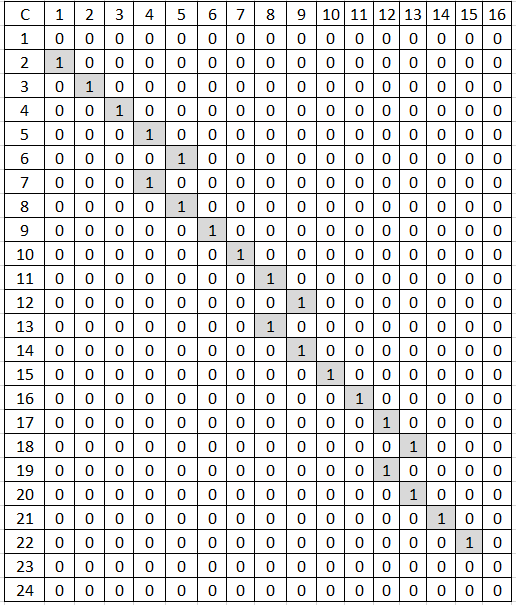
\includegraphics[width=0.5\textwidth]{./fig/CDmatrix.png}
    \caption{Mitral valve structure}
    \label{fig:CDmatrix}
\end{figure}
\begin{multicols}{2}
  \VerbatimInput[fontsize=\fontsize{7}{9}\selectfont]{Cmtxoutput.txt}
\end{multicols}
\newpage
\nosection{Coefficient matrix of equilibrium equations}
The matrix of the coefficients of the equilibrium equations for a ring element of a round plate is
given in the table.
  \begin{equation}\label{eqn:eqMatrix}
    [\overline{A}_k]=2\pi
    \begin{bmatrix}
        \rho_{k,1} & 0 & 0 & 0 & 0 & 0 \\[2ex]
        1.5\dfrac{\rho_{k,1}}{b_k}-1 & 1 & -2\dfrac{\rho_{k,1}}{b_k} & 0 & \dfrac{\rho_{k,1}}{2b_k} & 0 \\[2ex]
        -\dfrac{\rho_{k,2}}{b_k}+2 & -\dfrac{5}{6} & 2\dfrac{\rho_{k,2}}{b_k}-2 & \dfrac{2}{3} & -\dfrac{\rho_{k,2}}{b_k} & \dfrac{1}{6} \\[2ex]
        -\dfrac{\rho_{k,2}}{b_k} & -\dfrac{1}{6} & 2\dfrac{\rho_{k,2}}{b_k}2 & -\dfrac{2}{3} & -\dfrac{\rho_{k,2}}{b_k}-2 & \dfrac{5}{6} \\[2ex]
        0 & 0 & 0 & 0 & -\rho_{k,3} & 0 \\[2ex]
        \dfrac{\rho_{k,3}}{2b_k} & 0 & -2\dfrac{\rho_{k,3}}{b_k} & 0 & 1+1.5\dfrac{\rho_{k,3}}{b_k} & -1 \\[2ex]
      \end{bmatrix}
  \end{equation}
$A=[C]^T[\overline{A}]$ - equilibrium equation matrix, where:\par
$[C]^T$ - is transpose of compatibility matrix of displacements $[C]$\par
$[A]$ - is the matrix above in table\par
\smallskip
Calculation of the equilibrium equation matrix from Matlab\par
\VerbatimInput[fontsize=\fontsize{7}{9}\selectfont]{Amtxoutput.txt}
\newpage
\nosection{Flexibility matrix}
To reduce the size of the matrix and ease of placing it in the report, the equations were replaced
by j1, j2, j3, j4.
\begin{equation}\label{eqn:flexMatrix}
  [D_k]=\frac{2\pi b_k}{15K_k(1-\nu_k^2)}
  \begin{bmatrix}
        j_2 & -\nu_kj2 & 2j_1 & -2\nu_kj_1 & -\rho_{k,2} & \nu_k\rho_{k,2} \\[2ex]
            & j_2 & -2\nu_kj_1 & 2j_1 & \nu_k\rho_{k,2} & -\rho_{k,2} \\[2ex]
            &  & 16\rho_{k,2} & -16\nu_k\rho_{k,2} & 2j_3 & -2\nu_kj_3 \\[2ex]
            &  &  & 16\rho_{k,2} & -2\nu_kj_3 & 2j_3 \\[2ex]
            &  &  &  & j_4 & -\nu_kj_4 \\[2ex]
      \rlap{\textit{symm.}} &  &  &  &  & j_4 \\[2ex]
    \end{bmatrix}
\end{equation}
Where:\par
$K_k=\frac{E_kt_k^3}{12(1-\nu_k^2)}$
$j_1=\rho_{k,2}-b_k$\par
$j_2=4\rho_{k,2}-3b_k$\par
$j_3=\rho_{k,2}+b_k$\par
$j_4=4\rho_{k,2}+3b_k$\par
\smallskip
Calculation of the flexibility matrix from Matlab\par
\VerbatimInput[fontsize=\fontsize{7}{9}\selectfont]{Dmtxoutput.txt}

\newpage
\nosection{External load vector}
Vector of external forces for node described as:
\begin{equation}\label{eqn:ExtrLoad}
    \{F_k\}=
    \frac{2\pi b_k\rho_k}{3}
    \left\{\begin{matrix}
        3\rho_{k,2}-b_k \\[2ex]
        3\rho_{k,2}+b_k \\[2ex]
    \end{matrix}\right\}
    =
    \{\eta_k\}\rho_k
\end{equation}
$[F]=[F_o]+[C]^T[F_p]$, where:\par
$[F_o]=f_1 2\pi R_{f1} $\par
$f_1$ – value of external force which correspond $u_1$\par
$R_{f_1}$ - coordinate where is $m_1$\par
$[F_p]$ - represent the equivalent of distributed loads.\par
$[C]^T$ - is transpose of compatibility matrix of displacements $[C]$\par
{\noindent \footnotesize \verbatiminput{FOutput.txt}}
The results of global displacements are shown as following : 
\begin{equation}\label{eqn:Uglob}
    [U]=\{[A][D]^{-1}\}^{-1}[A]^T[F]
\end{equation}
Where:\par
$A$ - coefficient matrix of equilibrium equations\par
$[A]^T$ - transpose coefficient matrix of equilibrium equations\par
$[D]$: flexibility matrix\par
$[F]$ - External load vector\par
\begin{xtolerant}{300}{2em}
    {\noindent \footnotesize \verbatiminput{UglobOutput.txt}}
  \end{xtolerant}
\par
The results of internal forces are shown as following: 
\begin{equation}\label{eqn:Ulocal}
    [S]=[D]^{-1}[A]^T[U]
\end{equation}
Where:\par
$[D]$ - flexibility matrix \par 
$[A]^T$- transpose coefficient matrix of equilibrium equations\par 
$[U]$ - global displacements\par
%\begin{xtolerant}{300}{2em}
 %   {\noindent \footnotesize \verbatiminput{SOutput.txt}}
%  \end{xtolerant}
Results of internal forces ( S ) consists of $M_{\rho}$ and moments $M_{\varphi}$. 
Schema have 24 values of internal forces (S) it's divided
into: 12 values of moment $M_{\rho}$ and 12 values of moments $M_{\varphi}$. In the matlab command
$M_{\rho}=S(1:2:end)$ means to take the 1st value of (S) , 3rd , 5th , 7 th ..... till end. All
those values belong to moment $M_{\rho}$. For $M_{\varphi}=S(2:2:end)$ means to take the 2nd value
of (S), 4th , 6th.....till end.\par
\begin{xtolerant}{300}{2em}
    {\noindent \footnotesize \verbatiminput{M_Rooutput.txt}}
    {\noindent \footnotesize \verbatiminput{M_fioutput.txt}}    
  \end{xtolerant}
\newpage
\addcontentsline{toc}{section}{Internal forces and displacements}
\section*{Internal forces and displacements}
The equilibrium of finite element method used to solve the mentioned annular
plate. The results were obtained from a MATLAB commands. Based on these
calculations, the results shows the internal forces and the a distribution of
global displacements along our structure. The results shows that the maximum
displacement was U= 36.0471 mm in the direction gravity. The allowable
displacement was U.allowable = L/250 = 64 mm so, the verification was correct
based on the current geometry and material properties. Some parametric analysis
were done for plate thickness as a very important parameter to reduce the
displacement values.
\newpage
\nosection{Code listing}
\subsection*{Main function}
{\footnotesize \lstinputlisting[language=Matlab]{crplate.m}}
\subsection*{getAmtx function}
{\footnotesize \lstinputlisting[language=Matlab]{getAmtx.m}}
\subsection*{getDmtx function}
{\footnotesize \lstinputlisting[language=Matlab]{getDmtx.m}}
\newpage
%\printbibliography[title=List of literature]
\end{document}
